\documentclass[aspectratio=169]{beamer}

\usepackage[utf8]{inputenc}
\usepackage[spanish]{babel}
\usepackage{graphicx}
\usepackage{booktabs}
\usepackage{ragged2e}
\usepackage{minted}
\usepackage{xcolor}
\usepackage{tikz}
\usepackage{algorithm}
\usepackage{algorithmic}
\usepackage{minted}
\usepackage{listings}
\usepackage{tikz}
\usetikzlibrary{arrows.meta,positioning,fit,shapes.symbols}
\usetikzlibrary{arrows,shapes}
\definecolor{LightGray}{gray}{0.975}
\definecolor{links}{HTML}{2A1B81}
\hypersetup{colorlinks,linkcolor=,urlcolor=blue}
\AtBeginEnvironment{minted}{%
  \renewcommand{\fcolorbox}[4][]{#4}}

\usefonttheme{serif}

\usepackage{listings}
\lstdefinestyle{myCustomSQLStyle}{
  language=SQL,
  numbers=left,
  stepnumber=1,
  numbersep=10pt,
  tabsize=4,
  frame=single,
  backgroundcolor=\color{LightGray},
  breaklines=true,
  showspaces=false,
  showstringspaces=false
}

\newcommand\Wider[2][18mm]{%
    \makebox[\linewidth][c]{%
        \begin{minipage}{\dimexpr\textwidth+#1\relax}
            \raggedright#2
        \end{minipage}%
    }%
}

\title[ANN]{Emergent Digital Technologies}
\subtitle{Artificial Neural Networks (ANN)}
\author{Jiawei Han \& Jian Pei \& Hanghang Tong}
\date{\today}

% Remove navigation symbols...
\setbeamertemplate{navigation symbols}{}

\defbeamertemplate*{footline}{shadow theme}{
    \leavevmode
    \hbox{
        \begin{beamercolorbox}[
                wd =        0.33\paperwidth,
                ht =        2.5ex,
                dp =        1.125ex,
                leftskip =  0.3cm plus1fil,
                rightskip = 0.3cm
            ]{author in head/foot}
            \flushleft EDT
        \end{beamercolorbox}
        \begin{beamercolorbox}[
                wd =        0.33\paperwidth,
                ht =        2.5ex,
                dp =        1.125ex,
                leftskip =  0.3cm plus1fil,
                rightskip = 0.3cm
            ]{author in head/foot}
            \insertshorttitle
        \end{beamercolorbox}
        \begin{beamercolorbox}[
                wd =        0.33\paperwidth,
                ht =        2.5ex,
                dp =        1.125ex,
                leftskip =  0.3cm plus1fil,
                rightskip = 0.3cm
            ]{title in head/foot}
            \hfill \insertframenumber\,/\,\inserttotalframenumber%
        \end{beamercolorbox}
    }
}

\AtBeginSection[]{
    \begin{frame}<beamer>
        \frametitle{Plan}
        \tableofcontents[currentsection]
    \end{frame}
}

\newcommand{\toRight}[1]{
    \begin{FlushRight}
        {\tiny #1}
    \end{FlushRight}
}

\begin{document}

\frame{\titlepage}

\begin{frame}{Data Mining: Concepts and Techniques}
    \vspace{1mm}
    \centering
    
\includegraphics[height=0.65\textheight]{figures/book_cover.jpg} \\
    \vspace{1mm}
    {
        \scriptsize
        Content has been extracted from \textit{Data Mining: Concepts and Techniques}, by Jiawei Han \& Jian Pei \& Hanghang Tong. Morgan Kaufmann. 2022.
        Visit \url{https://shop.elsevier.com/books/data-mining/han/978-0-12-811760-6}.
    }
\end{frame}

\begin{frame}{Introduction to Artificial Neural Networks}
    \begin{itemize}
        \item Artificial Neural Networks (ANNs) are a family of techniques based on biological neural systems.
        \item A neural network is a set of connected input-output units where each connection has an associated weight.
        \item During learning, the network adjusts these weights to predict correct target values for input data.
        \item Applications include computer vision, natural language processing, and machine translation.
    \end{itemize}
\end{frame}

\begin{frame}{Introduction to Artificial Neural Networks (Cont.)}
    \centering
    
\includegraphics[width=0.9\textwidth]{figures/fig1}
\end{frame}

\begin{frame}{What is a Unit?}
    \begin{itemize}
        \item The basic building block of an ANN is the \textbf{unit}.
        \item Historically, basic classifiers like the perceptron and logistic regression are viewed as individual units.
        \item A unit is a mathematical function that:
        \begin{enumerate}
            \item Takes a linear weighted sum of the inputs.
            \item Passes that sum through an activation function $f(\cdot)$.
        \end{enumerate}
    \end{itemize}
\end{frame}

\begin{frame}{Mathematical Representation of a Unit}
    \begin{itemize}
        \item Given a data tuple $X = (x_1, x_2, \dots, x_n)$:
        \item \textbf{Net Input ($I$):} The linear weighted sum plus a bias scalar $b$.
        \[ I = \sum_{i=1}^{n} x_i w_i + b \]
        \item \textbf{Output ($O$):} The result of applying the activation function.
        \[ O = f(I) \]
        \item The bias $b$ acts as a threshold to adjust the net input of the unit.
    \end{itemize}
\end{frame}

\begin{frame}{Mathematical Representation of a Unit (Cont.)}
    \centering
    
\includegraphics[width=0.9\textwidth]{figures/fig2}
\end{frame}

\begin{frame}{Activation Functions}
    \begin{itemize}
        \item Activation functions are typically nonlinear.
        \item \textbf{Step Function:} Used in perceptrons; outputs 1 if $z \ge n$, else 0.
        \item \textbf{Sigmoid Function ($\sigma$):} Maps input to (0, 1).
        \[ \sigma(z) = \frac{1}{1 + e^{-z}} \]
        \item \textbf{ReLU (Rectified Linear Unit):} $f(I) = I$ if $I > 0$, and 0 otherwise.
        \item Nonlinearity allows ANNs to model complex, linearly inseparable data.
    \end{itemize}
\end{frame}

\begin{frame}{Activation Functions (Cont.)}
    \centering
    \includegraphics[height=0.85\textheight]{figures/af}
    \toRight{Source: The Click Reader (\url{theclickreader.com})}
\end{frame}

\begin{frame}{Multilayer Feed-forward Networks}
    \begin{itemize}
        \item This is a powerful and common type of ANN architecture.
        \item Consists of an \textbf{input layer}, one or more \textbf{hidden layers}, and an \textbf{output layer}.
        \item It is ``feed-forward'' because weights do not cycle back to previous units or layers.
        \item It is ``fully connected'' if each unit provides input to every unit in the next layer.
    \end{itemize}
\end{frame}

\begin{frame}{Layer Roles in ANN}
    \begin{itemize}
        \item \textbf{Input Layer:} Units correspond to the attributes of the input tuple and pass values unchanged.
        \item \textbf{Hidden Layers:} ``Neuron-like'' units that perform nonlinear transformations.
        \item \textbf{Output Layer:} Emits the final network predictions (e.g., class labels or numeric values).
        \item A ``two-layer'' network typically refers to one hidden layer and one output layer (input layer is not counted).
    \end{itemize}
\end{frame}

\begin{frame}{Feature Learning Hierarchy}
    \begin{itemize}
        \item Each layer learns features from the outputs of the previous layer.
        \item This creates a hierarchy of learned features at increasing levels of complexity.
        \item Example in Computer Vision:
        \begin{itemize}
            \item Input: Raw pixels.
            \item Layer 1: Edges.
            \item Layer 2: Contours/Corners.
            \item Layer 3: Object parts (e.g., wheels).
        \end{itemize}
    \end{itemize}
\end{frame}

\begin{frame}{The XOR Problem}
    \begin{itemize}
        \item The XOR problem involves four tuples: (0,1) and (1,0) are positive; (0,0) and (1,1) are negative.
        \item This dataset is \textbf{linearly inseparable}.
        \item A single linear classifier (perceptron) cannot separate the positive and negative tuples.
        \item This highlights the need for multilayer architectures with nonlinear activation.
    \end{itemize}
\end{frame}

\begin{frame}{Solving XOR with Neural Networks}
    \begin{itemize}
        \item A two-layer feed-forward network can solve XOR.
        \item Two hidden units can act as separate linear classifiers (perceptrons).
        \item The output unit combines these ``learned features'' to create a nonlinear decision boundary.
        \item This transforms the feature space into one where the tuples are linearly separable.
    \end{itemize}
\end{frame}

\begin{frame}{Solving XOR with Neural Networks (Cont.)}
    \centering
    
\includegraphics[width=0.9\textwidth]{figures/fig3}
\end{frame}

\begin{frame}{The Backpropagation Algorithm}
    \begin{itemize}
        \item A technique to automatically learn weights and biases from training data.
        \item It iteratively processes training tuples and compares predictions to known target values.
        \item Weights are modified to minimize the loss (e.g., mean-squared error).
        \item Modifications are made in the ``backward'' direction, from the output layer to the first hidden layer.
    \end{itemize}
\end{frame}

\begin{frame}{The Backpropagation Algorithm (Cont.)}
    \centering
    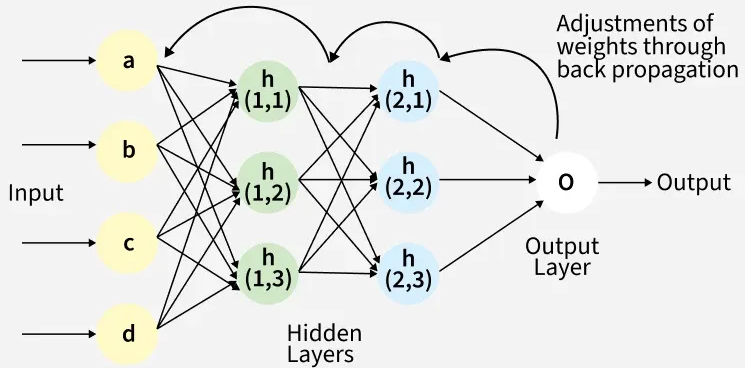
\includegraphics[width=0.75\textwidth]{figures/backpropagation}
    \toRight{\url{https://www.geeksforgeeks.org/machine-learning/backpropagation-in-neural-network/}}
\end{frame}

\begin{frame}{Phase 1: Forward Propagation}
    \begin{itemize}
        \item Inputs are fed to the network and pass through the input layer unchanged.
        \item For each unit in subsequent layers:
        \begin{enumerate}
            \item Compute net input: $I_j = \sum_i w_{ij} O_i + b_j$.
            \item Compute output: $O_j = f(I_j)$.
        \end{enumerate}
        \item Outputs are calculated layer by layer until the output layer provides a prediction.
    \end{itemize}
\end{frame}

\begin{frame}{Phase 2: Backward Propagation of Error}
    \begin{itemize}
        \item The error ($\delta$) is calculated starting from the output layer.
        \item For an output unit $j$ \footnote{assuming a \textit{sigmoid} activation function.}:
        \[ \delta_j = O_j(1 - O_j)(T_j - O_j) \]
        \item For a hidden unit $j$, error is a weighted sum of the errors of the units in the next higher layer ($l$):
        \[ \delta_j = O_j(1 - O_j) \sum_l \delta_l w_{jl} \]
    \end{itemize}
\end{frame}

\begin{frame}{Phase 3: Weight and Bias Updates}
    \begin{itemize}
        \item Parameters are updated using a gradient descent method.
        \item \textbf{Weight Update:} $w_{ij} = w_{ij} - \Delta w_{ij}$
        \[ \Delta w_{ij} = \eta \delta_j O_i \]
        \item \textbf{Bias Update:} $b_j = b_j - \Delta b_j$
        \[ \Delta b_j = \eta \delta_j \]
        \item $\eta$ is the \textbf{learning rate}, usually between 0.0 and 1.0.
    \end{itemize}
\end{frame}

\begin{frame}{The Backpropagation Algorithm (Cont.)}
    \centering
    
\includegraphics[width=0.70\textwidth]{figures/fig5}
\end{frame}

\begin{frame}{Weight Initialization}
    \begin{itemize}
        \item Weights and biases are initialized to small random numbers.
        \item \textbf{Breaking Symmetry:} It is critical that initial weights for units in the same layer are different.
        \item If weights are identical, units will always update in the same way.
        \item Random initialization ensures units can learn different features.
    \end{itemize}
\end{frame}

\begin{frame}{The Learning Rate ($\eta$)}
    \begin{itemize}
        \item The learning rate determines the size of the steps taken toward optimal weights.
        \item \textbf{Too Small:} Training is very slow.
        \item \textbf{Too Large:} Oscillation between inadequate solutions may occur.
        \item A common rule of thumb is to set $\eta = 1/t$, where $t$ is the number of iterations.
    \end{itemize}
\end{frame}

\begin{frame}{Gradient Descent vs. Stochastic Gradient Descent}
    \begin{itemize}
        \item \textbf{Gradient Descent (Full Batch):} Uses all training tuples to compute the gradient.
        \item \textbf{Stochastic Gradient Descent (SGD):} Updates parameters using a small ``mini-batch'' of tuples.
        \item SGD finds a direction that approximates the best direction.
        \item Overall, SGD is often much more computationally efficient.
    \end{itemize}
\end{frame}

\begin{frame}{Gradient Descent vs. Stochastic Gradient Descent (Cont.)}
    \centering
    \vspace{2mm}
    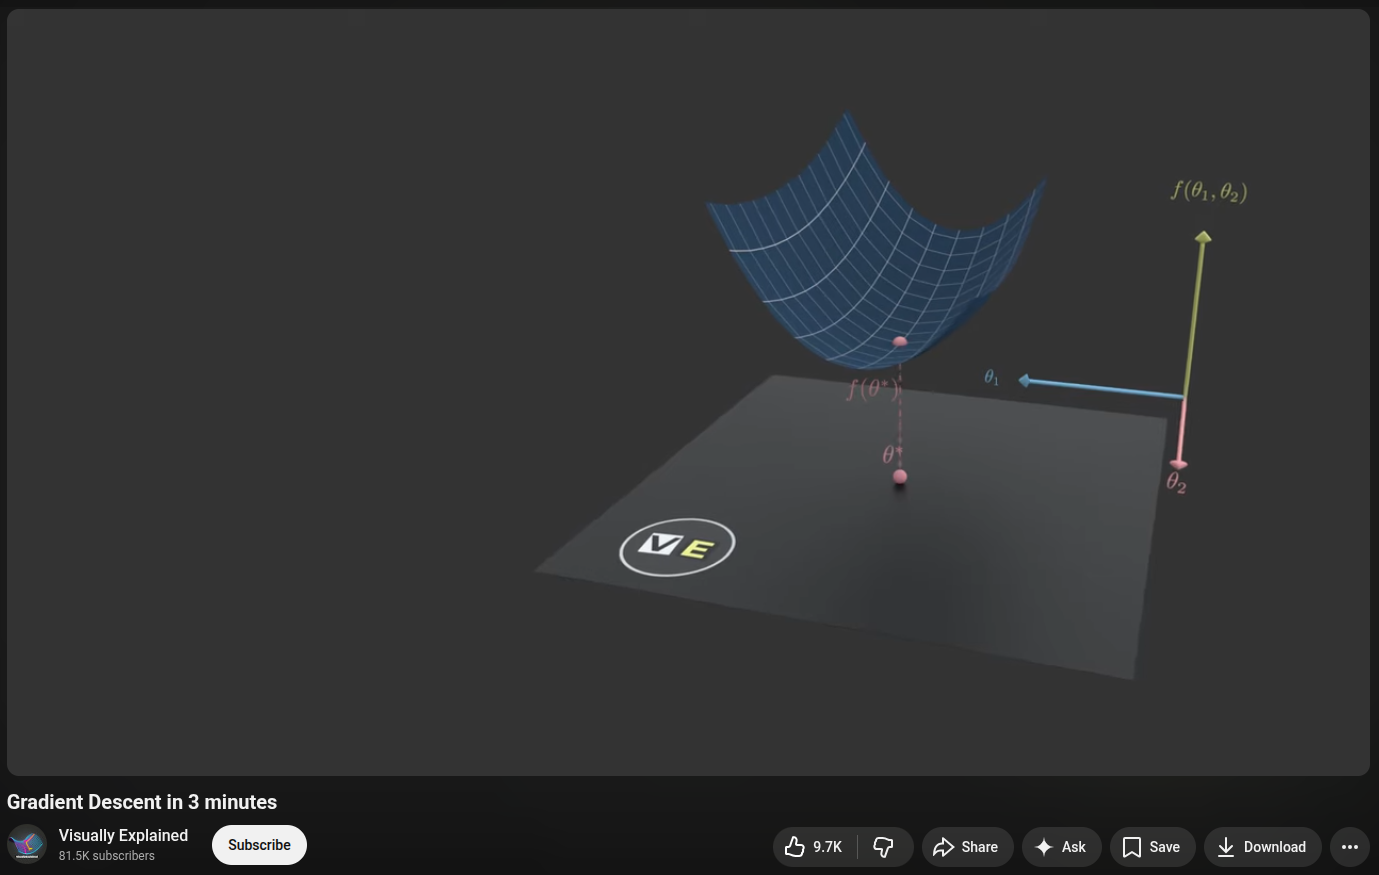
\includegraphics[width=0.75\textwidth]{figures/gradient}
    \toRight{\url{https://www.youtube.com/watch?v=qg4PchTECck}}
\end{frame}

\begin{frame}{Gradient Descent vs. Stochastic Gradient Descent (Cont.)}
    \centering
    \vspace{2mm}
    
\includegraphics[width=0.85\textwidth]{figures/fig6}
\end{frame}

\begin{frame}{Matrix Form Representation}
    \begin{itemize}
        \item Neural networks can be represented concisely using matrices.
        \item A layer transformation can be written as an \textbf{affine transformation}:
        \[ h_i = f(W_i h_{i-1} + b_i) \]
        \item $W_i$ is the weight matrix and $b_i$ is the bias vector.
        \item Matrix multiplication is often accelerated using GPUs instead of CPUs.
    \end{itemize}
\end{frame}

\begin{frame}{Optimization Challenges}
    \begin{itemize}
        \item Training error functions in ANNs are almost always \textbf{nonconvex}.
        \item Potential pitfalls include:
        \begin{itemize}
            \item \textbf{Local Minima:} Ending up in a high-cost area.
            \item \textbf{Plateaus:} Areas where the gradient is near zero.
            \item \textbf{Cliffs:} Areas with very large gradients.
            \item \textbf{Saddle Points:} Gradients are zero but it is not a local minimum.
        \end{itemize}
    \end{itemize}
\end{frame}

\begin{frame}{Optimization Challenges (Cont.)}
    \centering
    \vspace{2mm}
    
\includegraphics[width=0.85\textwidth]{figures/fig7}
\end{frame}

\begin{frame}{Generalization and Overfitting}
    \begin{itemize}
        \item The goal is to minimize the generalization error on unseen test tuples.
        \item \textbf{Overfitting:} Model fits training data perfectly but performs poorly on test data.
        \item Likely to happen with high model complexity and limited training samples.
        \item Effective training requires balancing optimization and generalization.
    \end{itemize}
\end{frame}

\begin{frame}{Data Mining: Concepts and Techniques}
    \vspace{1mm}
    \centering
    
\includegraphics[height=0.65\textheight]{figures/book_cover.jpg} \\
    \vspace{1mm}
    {
        \scriptsize
        Content has been extracted from \textit{Data Mining: Concepts and Techniques}, by Jiawei Han \& Jian Pei \& Hanghang Tong. Morgan Kaufmann. 2022.
        Visit \url{https://shop.elsevier.com/books/data-mining/han/978-0-12-811760-6}.
    }
\end{frame}

\end{document}
